\documentclass[a4paper, 12pt]{book}
\usepackage[margin=2.5cm]{geometry}
\usepackage[italian]{babel}
%\usepackage{wrapfig}
\usepackage{graphicx}   % per inserire immagini
\usepackage{caption}    % per le didascalie
\usepackage{subcaption} % per sottodidascalie

\usepackage{hyperref}
\usepackage{amsmath}
\setlength{\parindent}{0pt}
\usepackage{parskip}
\usepackage{soul}
\usepackage{xcolor}
\sethlcolor{yellow}
\usepackage{array}\usepackage[most]{tcolorbox}
\usepackage{booktabs}
\usepackage{tikz}
\usetikzlibrary{positioning}
\usepackage{longtable}
\usepackage{array}
\usepackage{fancyhdr}
\setlength{\headheight}{15pt}
\pagestyle{fancy}
\fancyhf{} % pulisce header e footer
\fancyhead[R]{\thepage} % numero pagina a destra nell'header
\renewcommand{\headrulewidth}{0pt} % (opzionale) elimina la riga orizzontale sotto l'header
\fancypagestyle{plain}{%
  \fancyhf{} % pulisce header e footer
  \fancyhead[R]{\thepage} % numero sempre in alto a destra
  \renewcommand{\headrulewidth}{0pt} % opzionale: niente linea
}
\setcounter{tocdepth}{3}

\title{\textbf{Basi di dati - primo semestre}\\uniVR - Dipartimento di Informatica}
\author{Mattia Nicolis \and Matteo Drago}
\date{A.A. 2025-26}

\begin{document}

    \maketitle

    \tableofcontents
    \markboth{}{}

    %-------MODULO DI TEORIA------------------------------------
    %-------Prof: Alberto Belussi-------------------------------
    %-------Lez: Martedì (10:30-12:30) [Aula A - Cav.1]----------
    %-------Lez: Venerdì (11:30-13:30) [Aula A - Cav.1]----------

    \chapter*{Introduzione}
    \addcontentsline{toc}{chapter}{Introduzione}

    \section*{Storia delle DBMS}
    \addcontentsline{toc}{section}{Storia delle DBMS}


    La nascita dei sistemi per la gestione di basi di dati ha visto due momenti principali:
    \begin{description}   % Ambiente description, [parola] in grassetto 
      \item [Anni '60:] Sviluppo di applicazioni negli \textbf{ambienti di ricerca scientifica}.
      \item [Anni '70:] Sviluppo di applicazioni informatiche in \textbf{ambito gestionale}.
    \end{description}

    Si trattava di semplici dispositivi in cui gli \underline{algoritmi} di elaborazione \underline{erano semplici} e \underline{grandi quantità di dati} erano \underline{\textbf{condivisi}} da più applicazioni.
    Queste caratteristiche erano specifiche per l'ambiente in cui erano state introdotte ovvero il \textbf{sistema informativo}.


  %------------BLOCCO DEFINIZIONE--------------------%

    \vspace{15pt}

    \begin{tcolorbox}[
      colback=cyan!5!white,
      colframe=blue!50!black,
      title=\textbf{Definizione - Sistema informativo},
      coltitle=white,
      fonttitle=\bfseries,
      arc=3mm,
      boxrule=0.5pt,
      enhanced,
      breakable
    ]
    L'insieme delle attività umane e dei dispositivi di memorizzazione ed elaborazione che organizza e gestisce l'informazione di interesse per una organizzazione di dimensioni qualsiasi.\\
    \textbf{N.B.: Non per forza è contenuta tecnologia informatica.}
    \end{tcolorbox}

    \vspace{15pt}

  %--------------------------------------------------%


    Il sistema informativo è costituito da \textbf{dati} e \textbf{informazioni}:
    \begin{description}
      \item [Dato:] elemento di conoscenza di base costituito da simboli che devono essere elaborati
      \item [Informazione:] interpretazione dei dati che permette di ottenere conoscenza più o meno esatta di fatti e situazioni.
    \end{description}
    
    Lo studio del sistema informativo avviene attraverso i diagrammi di flusso, questi permettono di svolgere diverse operazioni tra cui: 
    \begin{itemize}
      \item Definizione archivi dati e delle sorgenti di dati.
      \item Definizione degli utenti.
      \item Definizione di procedure e processi.
      \item Definizione dei flussi dati.
    \end{itemize}


    \clearpage
    \textbf{\large Come si è arrivati allo sviluppo dei DBMS?}
 
    Negli anni 70 i programmi comunicavano direttamente con i dati contenuti nel file system. Era una operazione scomoda in quanto l’accesso ai dati su file era scarso \textbf{(struttura ad accesso sequenziale)}, c'era ridondanza nei dati \textbf{(duplicazioni dello stesso dato su più file)}, inconsistenza dovuta ad aggiornamenti parziali e progettazione dei dati replicata per ogni programma.

    Negli anni 80 la soluzione che venne proposta fu quella di inserire un \textbf{DBMS} (Data Base Management System) tra il File System e le applicazioni.

    \begin{figure}[h]
      \centering

      \begin{subfigure}[b]{0.45\textwidth}
        \centering
        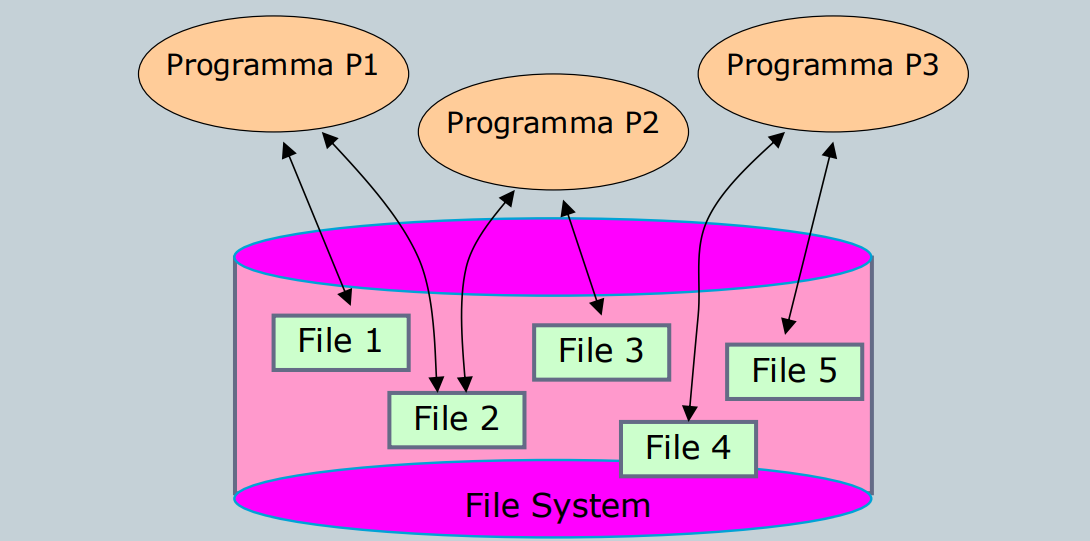
\includegraphics[width=\textwidth, height=3.8cm]{images/fileSystem.png}
        \caption{Solo file system}
      \end{subfigure}
      \hfill
      \begin{subfigure}[b]{0.45\textwidth}
        \centering
        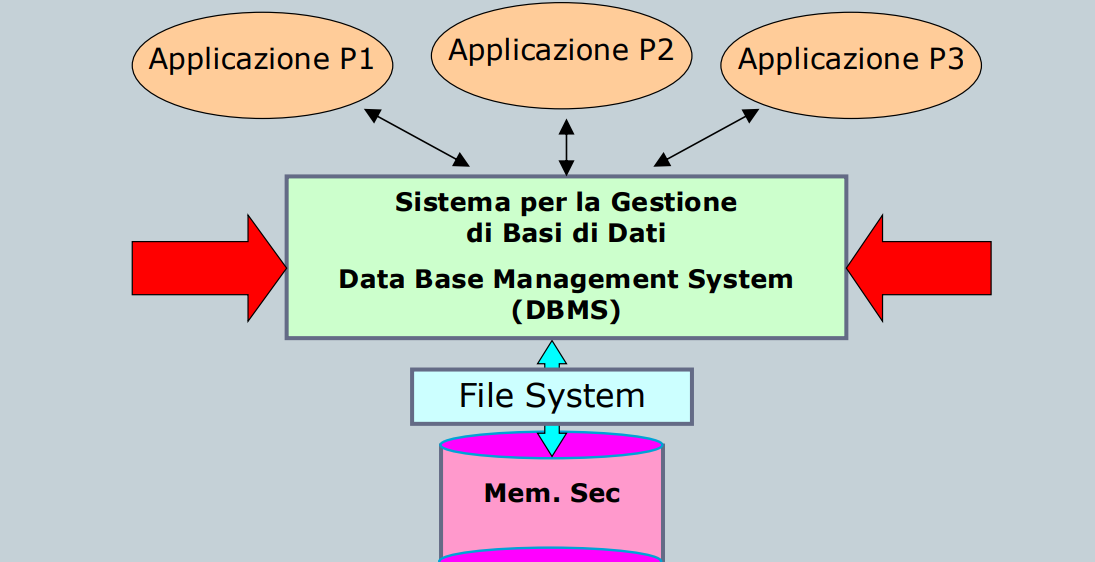
\includegraphics[width=\textwidth, height=3.8cm]{images/DBMS.png}
        \caption{File system + base di dati}
     \end{subfigure}

    \caption{Prima e dopo l'innovazione}
    \end{figure}



  %------------BLOCCO DEFINIZIONE--------------------%

    \vspace{15pt}

    \begin{tcolorbox}[
      colback=cyan!5!white,
      colframe=blue!50!black,
      title=\textbf{Definizione - Base di dati},
      coltitle=white,
      fonttitle=\bfseries,
      arc=3mm,
      boxrule=0.5pt,
      enhanced,
      breakable
    ]
    Una collezione di dati utilizzati per rappresentare con tecnologia informatica le informazioni di interesse per un sistema informativo.
    \end{tcolorbox}

    \vspace{15pt}

  %%%------------CHIUDE DEFINIZIONE-------------------%%% 

  %------------BLOCCO DEFINIZIONE--------------------%

    \vspace{15pt}

    \begin{tcolorbox}[
      colback=cyan!5!white,
      colframe=blue!50!black,
      title=\textbf{Definizione - DBMS},
      coltitle=white,
      fonttitle=\bfseries,
      arc=3mm,
      boxrule=0.5pt,
      enhanced,
      breakable
    ]
    Sistema che gestisce su memoria secondaria collezioni di dati \textbf{grandi, condivise} e \textbf{persistenti}, assicurandone \textbf{l'affidabilità, la privatezza e l'accesso efficiente.}
    \end{tcolorbox}

    \vspace{15pt}

  %%%------------CHIUDE DEFINIZIONE-------------------%%%  


    Questo nuovo approccio ha portato numerosi vantaggi:
    \begin{itemize}
      \item \textbf{maggiore astrazione} e più potenza espressiva per descrivere le proprietà del dato.
      \hl{All'interno del \textbf{DMBS} i dati vengono interpretati come oggetti ovvero istanze di classi o righe di tabelle}. Prima erano interpretati come blocchi o pagine di memoria secondaria (sequenze di byte)
      \item operazioni di accesso ai dati più complesse basate su un linguaggio di interrogazione (SELECT FROM WHERE) anzichè attraverso operazioni di READ/WRITE
      \item migliorata l'interazione uomo-informazione: 
      \begin{itemize}
        \item linguaggio per la definizione dei dati (Data Definition Language - DDL)
        \item linguaggio per l’interrogazione e aggiornamento dei dati (Data Manipulation Language – DML): 
        \begin{itemize}
          \item linguaggio di interrogazione: estrae informazioni da una base di dati (esempio: SQL, algebra relazionale)
          \item linguaggio di manipolazione: popola la base di dati, modifica il suo contenuto con aggiunte, cancellazioni e variazioni sui dati (esempio: SQL)
        \end{itemize}
      \end{itemize}
    \end{itemize}

    


   %------------BLOCCO DEFINIZIONE--------------------%

    \vspace{15pt}

    \begin{tcolorbox}[
      colback=cyan!5!white,
      colframe=blue!50!black,
      title=\textbf{Definizione - DBMS: modello dei dati},
      coltitle=white,
      fonttitle=\bfseries,
      arc=3mm,
      boxrule=0.5pt,
      enhanced,
      breakable
    ]
    È l’insieme dei costrutti forniti dal DBMS per descrivere la struttura e le proprietà dell’informazione contenuta in una base di dati.
    I costrutti permettono di definire le strutture dati che conterrano le informazioni e specificare le proprietà che dovranno soddisfare le istanze.

    \end{tcolorbox}

    \vspace{15pt}

  %%%------------CHIUDE DEFINIZIONE-------------------%%%  


     Nel passato esistevano modelli come quello reticolare o quello gerarchico. \\
     Attualmente si parla di modello relazionale, ad oggetti, object-relational (SQL99 o SQL3), basato sui documenti(JSON) o NoSQL


%------------BLOCCO DEFINIZIONE--------------------%

    \vspace{15pt}

    \begin{tcolorbox}[
      colback=cyan!5!white,
      colframe=blue!50!black,
      title=\textbf{Definizione - Schema di una base di dati},
      coltitle=white,
      fonttitle=\bfseries,
      arc=3mm,
      boxrule=0.5pt,
      enhanced,
      breakable
    ]
    È la descrizione della struttura e delle proprietà di una specifica base di dati fatta utilizzando i costrutti del modello dei dati (lo schema di una base di dati è invariante nel tempo).

    \end{tcolorbox}

    \vspace{15pt}

  %%%------------CHIUDE DEFINIZIONE-------------------%%%  

  %------------BLOCCO DEFINIZIONE--------------------%

    \vspace{15pt}

    \begin{tcolorbox}[
      colback=cyan!5!white,
      colframe=blue!50!black,
      title=\textbf{Definizione - Istanza di una base di dati},
      coltitle=white,
      fonttitle=\bfseries,
      arc=3mm,
      boxrule=0.5pt,
      enhanced,
      breakable
    ]
    È costituita dai valori effettivi che in un certo istante popolano le strutture dati della base di dati (l’istanza di una base di dati varia nel tempo).

    \end{tcolorbox}

    \vspace{15pt}

  %%%------------CHIUDE DEFINIZIONE-------------------%%%  


    \begin{figure}[h]
        \centering
        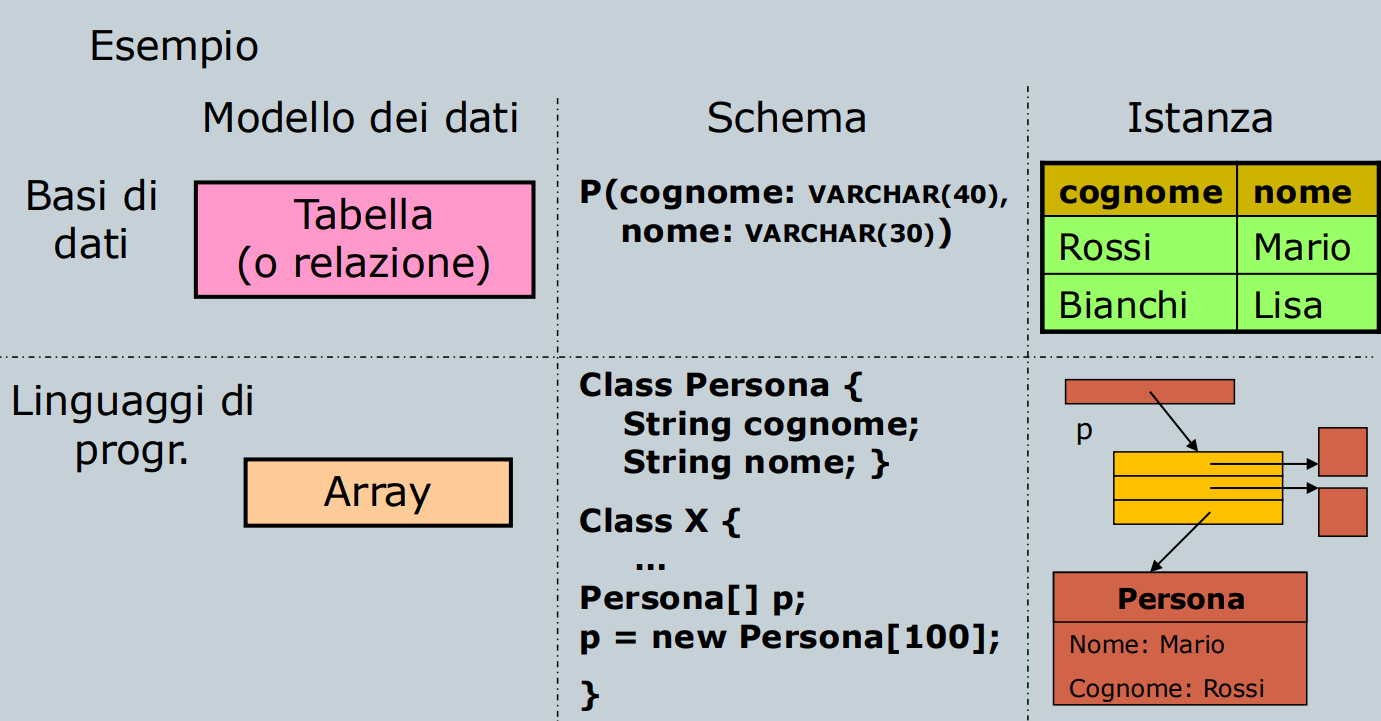
\includegraphics[width=0.8\textwidth]{images/modelloSchemaIstanza.png}
        \caption{Distinzione tra modello, schema e istanza}
    \end{figure}



    \section*{Architettura di un DBMS}
    \addcontentsline{toc}{section}{Architettura di un DBMS}

    \begin{itemize}
      \item \textbf{Schema Logico:} è la rappresentazione della struttura e delle proprietà della base di dati definita attraverso i costrutti del modello dei dati del DBMS.
      \item \textbf{Schema Interno:} è la rappresentazione della base di dati per mezzo delle strutture fisiche di memorizzazione (file dati, file indice, ecc…).
      \item \textbf{Schema Esterno:} descrive una porzione dello schema logico di interesse per uno specifico utente o applicazione (attraverso viste sullo schema logico).\\
    \end{itemize}
  
    
    La caratteristica fondamentale di queste strutture è \textbf{l'indipendenza}.
    \begin{description}
      \item[Indipendenza FISICA:] lo \underline{schema logico} della base di dati \underline{è completamente indipendente dallo schema interno}, ne consegue che le variazioni delle strutture fisiche non impattano sullo schema logico e quindi sulle applicazioni.
      \item[Indipendenza LOGICA:] gli \underline{schemi esterni} della base di dati \underline{sono indipendendi dallo schema logico}, ne consegue che le variazioni dello shcema logico (purchè non vengano rimossi dati) non impattano sugli schemi esterni e quindi sulle applicazioni (eventualmente è necessario solo ridefinire l'espressione di derivazione).
    \end{description}
     

    \section*{Progettazione di una base di dati}
    \addcontentsline{toc}{section}{Progettazione di una base di dati}
  

    \dots


\end{document}
